\chapter{Webbdatabas för hantering av filer}

\section{Systemarkitektur}
I inledningen av projektet hölls en diskussion om hur systemet skulle utvecklas. Faktorer som språk och ramverk togs upp. Beslutet som fattades var att språket Ruby och ramverket Ruby on rails skulle användas som grundstomme i projektet. Vidare användes också Javascript och ramverket Angularjs för att göra upplevelsen av systemet snabbare för användaren.

\subsection{Ruby och Ruby on rails}
Ruby on rails är ett ramverk skrivet i språket Ruby \cite{rubylang}. Det är ett ramverk med öppen källkod som används utav flera stora tjänster på nätet, bland andra mikrobloggstjänsten Twitter, sammarbetsverktyget Github och boendeförmedlingstjänsten Airbnb. Ramverket är skrivet enligt designmönstret MVC. Detta står för \textit{model}, \textit{view}, \textit{controller} och är ett sätt att strukturera ett projekts logik på sådant vis att olika komponenter har sin egna tydliga plats och syfte.

I Ruby on rails skapar utvecklaren \textit{models}. Detta är en samling klasser vars syfte är att hantera data som användaren eller systemet interagerar med, och fungerar som ett lager ovanpå databasen. Ett exempel på en \textit{model} kan vara en klass för användare eller filer. Genom dessa klasser hanteras all information om just användare respektive filer, och samtliga databasoperationer sker genom klassernas metoder.

Den komponent som sköter interaktionen mellan användare och systemets \textit{models} är systemets \textit{controllers}. Här finns logik för att hantera användares handlingar och hämta data från systemets \textit{models}. Ett exempel kan vara att användaren klickar på en knapp i webbläsaren. Syftet med knappen är att visa en viss data. Användarens handling skickas till en \textit{controller} som tar emot vad det är för data som användaren efterfrågar och hämtar den datan från en \textit{model}. Här kan också logik för att hantera undantag, till exempel att datan saknas, finnas. Den \textit{controller} som anropats skickar sedan resultatet av användarens begäran vidare till användaren.

Det som användaren i sin tur interagerar med är systemets \textit{views}, på svenska vyer. Här presenteras det som systemets \textit{controllers} producerat. Knappen som användaren trycker på i exemplet i stycket ovan skapas i en \textit{view}. Här kan också finnas länkar, texter, textfält och alla andra komponenter som utgör det som renderas av en webbläsare.

En mer överskådlig figur för hur data och interaktioner generellt sett färdas genom ett MVC-system visas i figur \ref{fig:mvc1}. Data transporteras från \textit{models} till \textit{views} via \textit{controllers}. Interaktioner färdas mellan \textit{views} och \textit{models} via \textit{controllers} och direkt mellan \textit{controllers} och \textit{views} samt mellan \textit{controllers} och \textit{models}.

\begin{figure}[!H]
\centering
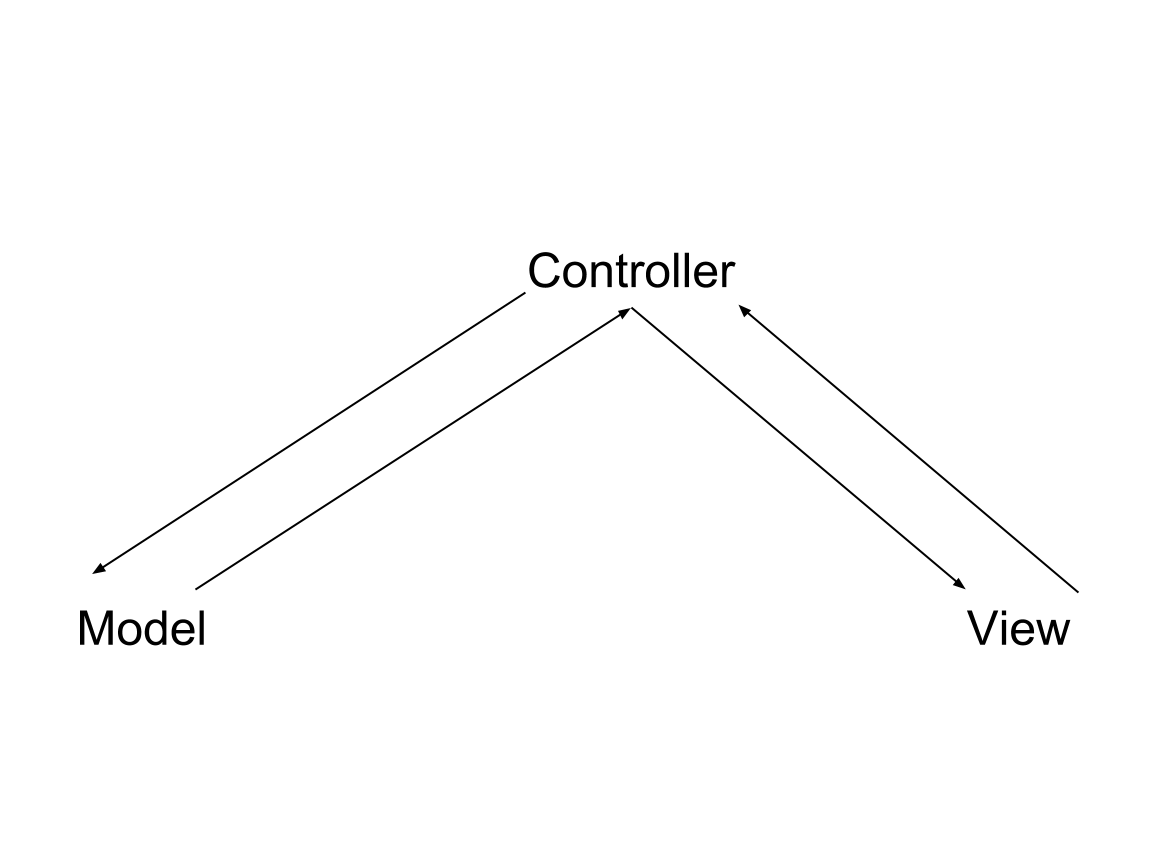
\includegraphics[width=0.8\textwidth]{figures/mvc1.png}
\caption{Visar på dataflödet i ett MVC-system}
\label{fig:mvc1}
\end{figure}

En annan figur som snarare fokuserar på MVC ur ett användarperspektiv visas i figur \ref{fig:mvc2}.

\begin{figure}[!H]
\centering
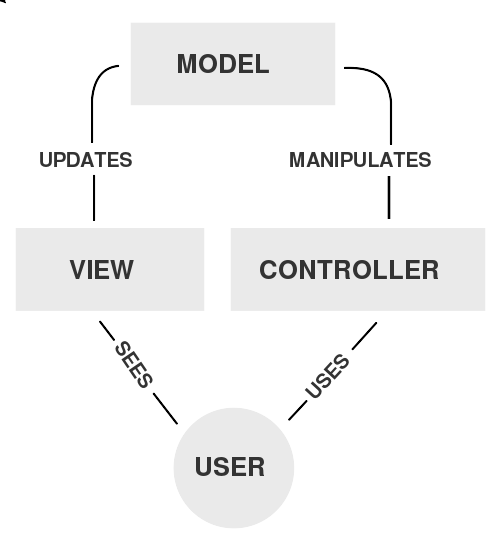
\includegraphics[width=0.8\textwidth]{figures/MVC_wiki.png}
\caption{Visar på MVC-flödet ur ett användarperspektiv.}
\label{fig:mvc2}
\end{figure}

Fördelarna med att använda ett webbramverk som Ruby on rails eller motsvarande är flera, och kan generaliseras med att säga att det är onödigt att uppfinna hjulet på nytt. Säkerhet, effektivitet och struktur är aspekter som förstärks utav Ruby on rails. En mer konkret fördel med Ruby on rails är klassen \emph{ActiveRecord} som alla modeller i systemet ärver av. \emph{ActiveRecord} har funktioner för att hantera relationer och frågor mot databasen. Mer om \emph{ActiveRecord} och databashantering i kapitel \ref{ssec:activerec}.

\subsection{Javascript och Angularjs}
För att skapa ett responsivt system, i bemärkelsen att det var snabbt för användaren, valdes det att implementera mycket utav funktionaliteten hos klienten med hjälp av Javascript. Systemet innehåller många olika komponenter som ska interagera med varandra. Ett exempel är då flera filer ska listas med verktyg för att hantera filen, samtidigt som den filen har flera taggar som också ska kunna hanteras.

Ramverket Angularjs valdes bland annat på grund av dess stöd för så kallade templates men även för dess tvåvägsbindning för variabler. Tvåvägsbindningen gjorde det enklare att utveckla komponenter som beror på hur användaren interagrerar med textfält eller knappar. Till exempel krävdes det väldigt lite ansträngning för att uppdatera en rubrik till det som användaren skrev i ett textfält samtidigt som denne skrev, eller att uppdatera både textfältet och rubriken samtidigt.

Angularjs är ett så kallat MVW-ramverk, vilket står för \textit{Model-View-Whatever} \cite{angularjs}. För att effektivt använda detta ramverk bör även systemet byggas upp efter den designen. Då \textit{whatever} innebär att det finns flera olika typer av sätt att kontrollera eller manipulera data på kan varje komponent i systemet få specialanpassade lösningar.

\section{Tredjepartsmjukvara}
Då Ruby on rails och Angularjs är mjukvara med öppen källkod har det bildats globala nätverk kring dessa ramverk. Många tillägg, verktyg och bibliotek har skrivits för att underlätta utvecklandet i dessa ramverk. För att fortsätta bidra till detta nätverk utvecklades även projektet med hjälp av öppen källkod, för att kunna dela de lösningar som tagits fram.

För att underlätta för utvecklare har Ruby on rails byggts med många verktyg för utvecklare. Möjligheten finns även för utvecklare att bygga egna verktyg som kallas för \textit{gems} och är ofta fria att använda och även de är skrivna med öppen källkod. Några som använts under utvecklandet av detta system är:

Byebug, ett avlusningsverktyg som möjliggör för utvecklare att sätta brytpunkter i koden. När systemet kör och stöter på den rad där denna brytpunkt finns pausas systemet. I konsolen kunde sedan variabler granskas och utvecklarna kunde steg för steg följa vilken väg koden följde.

Letter opener, ett verktyg för att hantera e-post som skickas av systemet. Istället för att utvecklaren sätter upp en e-postserver som skickar e-postmeddelandena på riktigt öppnar Letter opener mailen i webbläsaren. Detta gjorde att utvecklingen av systemets e-postrelaterade komponenter blev betydligt enklare.

För utvecklandet av Angularjs och annan Javascript användes Chrome developer tools och tillägget Angularjs batarang. Dessa är verktyg som gör det lättare för utvecklare att följa med i vad som händer då de använder webbläsaren Google chrome. Med funktioner som brytpunkter och möjligheten att bevaka variabler blir utvecklandet betydligt enklare.

\section{Filhantering}
För att hantera tjänstens filer implementerades tre olika fillagringssätt. En modulär filhantering skapades för att lätt kunna implementera fler sätt att lagra filer. Dropbox implementerades först eftersom det ansågs vara ett enkelt sätt att hantera användarens filer. När det väl implementerats upptäcktes det att Dropbox krävde en krypterad anslutning till systemet, vilket kostar pengar. På grund av detta infördes även Google drive som lagringssätt. Efter ett möte med kunden flyttades fokus till att också implementera lokal fillagring.

\subsection{Dropbox}
Dropbox implementerades med hjälp av Dropbox SDK. SDK står för \textit{Software Development Kit} vilket är en uppsättning av utvecklingsverktyg för mjukvaruutveckling mot specifika ramverk eller programpaket, i det här fallet till utveckling mot Dropbox tjänster. Dropbox SDK ger verktyg för att utveckla nya tjänster som använder sig av Dropbox olika funktioner. Webbtjänsten som utvecklades använder sig av ned- och uppladdning av filer till och från Dropbox. För att nå användarens filer måste en autentisering till Dropbox ske, vilket görs med hjälp av Omniauth, en \textit{gem}. Med hjälp av Dropbox SDK hämtas metadata för filerna i rot-mappen för att sedan visas för användaren. Om en mapp sedan blir klickad på hämtas metadatan för filerna i den mappen med hjälp av sökvägen. En fil laddas också ned med hjälp av dess sökväg. För att ladda upp filer till Dropbox krävs det att de läggs till i en existerande mapp eller i rot-mappen. För att hålla filerna som laddats upp från tjänsten till Dropbox samlade, skapades först en mapp i Dropbox dit filerna laddades upp till.

\subsection{Google drive}
Likt Dropbox användes Google drives SDK för att kunna använda deras funktionalitet i systemet. För att nå användarens filer krävs en autentisering för att ansluta till användarens konto hos Google drive. Det här görs med hjälp av två \textit{gems}, Drive SDK samt Omniauth. Filhanteringen sker likt metoden för Dropbox förutom att Drive inte strukturerar sina filer med hjälp av sökvägar. Varje fil har istället en parameter för \textit{parent} och varje mapp har en parameter \textit{child}, där eventuella filer i mappen lagras. Om en fil ligger i en mapp är mappen filens \textit{parent} och filen är mappens \textit{child}. För att identifiera det här förhållandet kommer alla filer som ligger i samma mapp ha mappens id i dess \textit{parent} parameter. Liknande kommer mappens parameter \textit{child} innehålla alla id tillhörande filer som ligger i mappen, se figur \ref{fig:parentchild}.

\begin{figure}[!H]
\centering
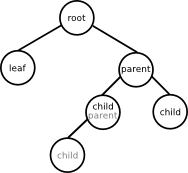
\includegraphics[width=0.8\textwidth]{figures/parentchild.png}
\caption{Visar strukturen för parametrarna \textit{parent} och \textit{child} i Google drive.}
\label{fig:parentchild}
\end{figure}

\subsection{Lokal fillagring}
Den lokala filhanteringen infördes för att ge användaren ett alternativ utan extern kostnad och utan filutrymmesbegränsningar från externa tjänster. För att sköta uppladdningen, som är en central del av den lokala filhanteringen i och med att det inte går att importera filer likt från Google drive eller Dropbox, implementerades en så kallad drag och släpp-uppladdning. Detta innebär att användaren kan markera en eller flera filer på sin dator, och dra dem till webbläsarfönstret där systemet är öppet, och släppa dem där. Systemet tar där vid och laddar upp filerna. När servern har tagit emot all uppladdningsdata från webbläsaren får filen ett slumpat filnamn och placeras i en mapp på servern.

\section{Hantering och strukturering av databaser}
Systemet använder sig utav en SQL-databas, där SQL står för \textit{Structured Query Language}. Det är ett programmeringsspråk för att lagra, bearbeta och hämta information i en databas \cite{sqlenc}.

\subsection{Databasstruktur}
\label{ssec:activerec}

Inledningvis i projektet hölls ett möte för att ta fram en grundläggande databastruktur. Denna innehöll användare, användares olika externa konton (till exempel Dropbox eller Google Drive), filer och nyckelord. Vidare skapades också en tabell som länkade samman filer och nyckelord.

\subsection{Databashantering}

En stor komponent utav Ruby on Rails är modulen som heter \texttt{ActiveRecord}. Detta är en modul vars syfte är att abstrahera och förenkla databashantering \cite{objrel} och skapades efter ett designmönster med samma namn \cite[kapitel 1]{proar}. Istället för att skriva databasfrågor manuellt kan du använda systemets \texttt{ActiveRecord}-modeller för att förenkla arbetet. Rent praktiskt kan detta innebära att ersätta \texttt{SELECT * FROM table WHERE column1=’value’} med \texttt{Table.where(column1: ‘value’)}.

Fördelen med detta var att komplexa relationer mellan olika tabeller kunde förenklas, och en objektorienterad struktur med Rubyklasser skapades utifrån tabellerna. En extern nyckel i en SQL-tabell kan i sin \texttt{ActiveRecord}-form liknas med en pekare till ett annat objekt. Detta ledde till att arbetet kunde skyndas på, och att avancerad kunskap om SQL-frågor inte var nödvändigt.

I och med att Rails \texttt{ActiveRecord}-modul hade inbyggt stöd för SQL-databaser användes dessa för systemets relationella tabeller. Mer specifikt användes Postgresql i systemet. En fördel med Postgresql är dess indexering som bygger på bland annat B-trees \cite{indexes}. (Redogörelse för indexeringsmetoder och datastrukturerna bakom dem går bortom räckvidden för denna rapport.) Denna indexeringsmetod möjliggjorde snabba sökningar baserat på olika parametrar (exempelvis namn eller etiketter), vilket ansågs viktigt för systemet.

\section{Gränssnitt}

...

\section{Testning}

Sedan version 1.9 utav Ruby har standardverktyget för testning varit Minitest \cite{rubychangelog}. Minitest erbjuder många delar som behövs för att kunna hantera testning. Det som användes mest var så kallade fixtures, en datarepresentation utav en model i systemet. Dessa användes för att säkerställa att systemet producerade de förändringar mot modellen som var väntade. Men även att de controllers som fanns i systemet utförde rätt logik beroende på datan.

För att kontinuerligt säkerställa att projektet levde upp till de krav testerna specificerade användes build-servern Travis CI. Varje gång ny kod laddades upp gavs då ett resultat om hur testerna gick. Med denna kontinuerliga uppdatering går det att via GitHub följa projektets status utan att ladda ned och starta det.

För testning av gränssnittet krävs dock en renderingsmotor för Javascript. Då den valda build-servern redan hade en motor som heter Phantomjs installerat valdes den. För att integrera Phantomjs med Minitest användes Capybara. Capybara är ett testningsverktyg och finns som tillägg till Minitest. Capybara erbjuder inte bara stöd för rendering utav javascript med Phantomjs utan ger också hjälpfunktioner för end-to-end testning.

Tester skrevs efter att en funktion hade implementerats för att säkerställa att den önskade funktionaliteten skulle hålla i framtida utveckling av andra funktioner.

\section{Utvecklingsmetodik}

Genom att följa en bra utvecklingsmetodik gavs en bra grund och tydliga riktlinjer att följa under projektets gång. Den utvecklingsmetodik som låg till grund för projektet var Scrum \cite{scrumguide}. Scrum är ett ramverk som innefattar olika roller, aktiviteter och tekniker för förenkla utvecklingsprocessen. Det finns nyckelroller inom teamet för att se till att alla delar ses över utan att lägga allt ansvar på en individ. Det finns även en rad förutbestämda möten och uppdateringar som är till för att ge hela gruppen bra överblick och en chans att påverka arbetet.

Utvecklingsteamet bestod av fem personer där varje person fick en nyckelroll:

\begin{itemize}
  \item Scrummästare: Dennes ansvar innefattade att se till att teamet höll sig till de riktlinjer som fanns, sköta kommunikationen runt de mer administrativa bitarna (boka sal, bestämma arbetsdagar och så vidare) och hålla i scrummöten.
  \item Produktägare: Produktägarens ansvar var att hålla kontakten med kund och se till att kundens krav omvandlades till scenarion och uppgifter. Det var även dennes ansvar att hålla ordning i produktbackloggen som är den lista där alla scenarion sparas.
  \item Kodansvarig: Dennes ansvar gick ut på att hitta ett bra system för att integrera nya delar i det befintliga systemet och sedan se till att detta system upprätthölls.
  \item Testansvarig: Dennes uppgift var att se till att systemet testades för att säkerställa att de krav som fanns uppnåddes och för att kontinuerligt jobba för att upptäcka brister i systemet.
  \item Dokumentansvarig: Dokumentansvarig hade till uppgift att säkerställa att projektet blev ordentligt dokumenterat. Det var önskvärt att ha protokoll från kundmöten, teammöten med beslutsfattande karaktär och dokumentera skisser och liknande vid diskussioner kring systemets uppbyggnad.
\end{itemize}

Hela utvecklingsperioden delades upp i mindre tidsrutor, så kallade sprints. Dessa sprints hade en förutbestämd tid som inte kunde förlängas även om teamet upplevde att tiden inte räckte till. Varje sprint hade samma struktur. Vid uppstart hölls en sprintplanering där alla i teamet satte sig tillsammans för att gå igenom vilka scenarion från produktbackloggen som skulle ligga till grund i förestående tidsperiod. Det var viktigt att försöka hålla en god balans mellan tid och antalet valda scenarion. Teamet fick tillsammans utvärdera om de ansåg det möjligt att utföra alla scenarion innan sprintens avslut. När samtliga scenarier var valda bröts de ned i mindre delar och formades till specifika uppgifter. Det var önskvärt att hålla dessa uppgifter små och konkreta för att ha möjlighet att genomföra dessa under en arbetsdag.

Inför varje arbetsdag i en sprint höll teamet ett dagligt scrummöte. Detta var ett kort möte på max 15 minuter där alla i teamet stod upp, utan datorer. Detta för att hålla mötet kort och fokuserat. Varje individ fick under detta möte berätta vad de gjorde senast och vad de skulle göra denna kommande dag. Detta gav alla en bra inblick i arbetet och en kort avstämning på hur teamet låg till tidsmässigt.

Den sista arbetsdagen i varje sprint ägnades åt två avslutande möten. Det första av dessa var en sprintgranskning. Detta var ett tillfälle då hela teamet kunde diskutera det senaste projektinkrement och hur arbetet hade fortskridit. Det första som gjordes på dessa möten var att gå igenom de scenarion som fanns inför sprinten och om dessa blivit avslutade. Eftersom målet med varje sprint var att ha en fungerande produkt med de krav som scenarierna representerade uppfyllda, gav denna genomgång en tydlig bild huruvida sprintmålet uppnåtts eller inte. Nästa del i mötet var att diskutera de problem som uppstått under sprintens gång och hur dessa blivit lösta. Återstoden av dessa möten ägnades åt att diskutera den dåvarande backloggen, vad som skulle göras härnäst och vilka variabler som fanns inför nästa produktinkrement.

Den sista aktiviteten i varje sprint var en sprintåterblick. Detta var ett möte där gruppen lade fokus på sina egna prestationer, de sociala relationerna i gruppen och de verktyg som använts. Detta var ett tillfälle där alla fick möjlighet att yttra och påverka dessa aspekter för att jobba mot ett bättre arbetsklimat.

För att kunna skapa en realistisk bild över projektets storlek, vilka tidsramar projektet skulle delas upp i och hur mycket som skulle kunna åstadkommas under projektets gång skapades en tidsplan. För att ge en tydlig bild skapades ett Gantt-schema \cite{softwareeng} i ett Google sheet i teamets gemensamma Google Drive. Där samlades alla dagar i projektperioden. I schemat kunde deadlines, tänkta kundmöten, sprintarna och lediga perioder åskådliggöras på ett smidigt sätt. [BILAGA?!?!]

Här presenteras kort det fokus som fanns för varje sprint. Fullständiga sprintbackloggar går att se i [APPENDIX!!=!=?!].

\subsection{Sprint 1 - MVP}

Målet med denna sprint var att ha en \emph{Minimal Viable Product}, MVP [KÄLLA] efter sprintavslutet. Något som var funktionellt och kunde visa på de problem som systemet skulle kunna lösa i ett senare skede. Fokus låg på att skapa en användare med Dropbox som fildatabas, importera filer från Dropbox till systemet och skapa nyckelord för filerna.

\subsection{Sprint 2 - Utveckla den tekniska funktionaliteten}

Fokus här var att göra filerna lättåtkomliga och sökbara. Dock stöttes det på ett problem gällande Dropbox som fildatabas. En kostnad för HTTPS-certifikat gjorde att teamet fick ändra riktning efter samråd med kund. Utöver sökningen blev det även fokus på att skapa ett mer modulärt system för att kunna lägga till flera typer av databaser. Det teamet kom överens om var att implementera Google Drive och även skapa en lokal databas för egen server. Då förändringar ledde till ett väldigt spretigt och icke målbaserat arbete valdes det att avsluta denna sprint i förtid.

\subsection{Sprint 3 - Tänka på användaren}

Under sprint tre hamnade fokus mer på systemets användare än den tekniska funktionaliteten. Ett flöde för systemet togs fram [BILD?], sökresultatens visning diskuterades [BILD?] samt utvecklades, och funktionalitet för drag-och-släpp-uppladdning påbörjades.

\subsection{Sprint 4 - Färdig produkt}

I denna sista sprint var det önskvärt att skapa ett användargränssnitt, få klart alla öppna scenarion och förbättra redan implementerad kod.

\section{Versionshantering och kodgranskning}

För versionshantering användes Git i kombination med Github genomgående i projektet. Git är ett distribuerat versionshanteringssystem där samtliga utvecklare har en komplett lokal kopia av hela projektet på dess egna datorer \cite[kapitel 1.1]{progit}. Detta underlättade för en agil utveckling där målet var att alltid ha en fungerande produkt.

För att underlätta vid konflikter och andra problem som uppstår då parallell utveckling av närliggande delar av projektet skedde användes Gits förgreningsfunktion. Förgreningar är en metod för att lösa problem som uppstår vid en linjär utveckling, där allt måste ske i en viss ordning. Flera utvecklare kunde jobba på olika komponenter utifrån en gemensam grund, och Git höll sedan koll på hur dessa kunde sammanfogas på enklast möjliga vis \cite[kapitel 3.1]{progit}.

Inom förgreningen implementerades också en metodik som populärt kallas \emph{feature branches} – funktionalitetsgrenar \cite[kapitel 16]{gitflow}. Då en ny funktionalitet skulle implementeras i systemet skapade den ansvarige utvecklaren en förgrening. När utvecklaren var klar med det den jobbade med, skapades en förfrågan på GitHub (en \emph{pull request}) om att sammanfoga koden för den nya funktionaliteten med den befintliga. Innan koden sammanfogades fick den ansvarige utvecklaren återkoppling från resterande medlemmar i utvecklingsteamet om de blivande förändringarna och tilläggen. På så sätt skapades en trygghet för utvecklargruppen att det fanns en gemensam förståelse och konsensus kring det som skulle bli en del av den befintliga kodbasen.

